\section{$\beta$-$\gamma$ irradiator}
\label{sec:irradiador}
In order to carry out experiments with radiation,
we built an apparatus which allows us to expose samples to 
precise doses of $\beta$ and $\gamma$ rays,
while keeping the operator shielded.
The apparatus consists of a lead tube lined with PVC on its inner wall
(\figref{fig:corteirradiador}).
\fig{corteirradiador}{figuras/poster/corte.pdf}{Cutaway drawing of the irradiator}

All surfaces which might be exposed to $\beta$ particles are covered in PVC,
to stop the particles while producing the least possible amount of braking
X rays.

Near one end of the cavity is a \Strontium source
(\figref{fig:fuente})
\fig{fuente}{figuras/poster/fuente.pdf}{Cutaway drawing of the \Strontium $\beta$ source.}
in a plastic pocket attached to a rotating lead block
(\figref{fig:piezagiratoria}).
\fig{piezagiratoria}{figuras/poster/piezagiratoria.png}
{Rotating assembly where the $\beta$ source is mounted.}
When the lead is interposed between the $\beta$ source and the inside of the cavity,
it is safe for people to open the cavity and handle the samples inside
(\figref{fig:posicionno}).
When the assembly is rotated towards the other side,
the $\beta$ source emits radiation into the cavity without any obstacles
(\figref{fig:posicionsi}).

The assembly was motorized by Javier Badía as part of his final annual laboratory course.
This allows for exposure to be controlled with a switch (or a computer program)
in a simple, fast and repeatable manner.
\begin{figure}[H]
    \centering
    \begin{subfigure}[b]{.45\textwidth}
        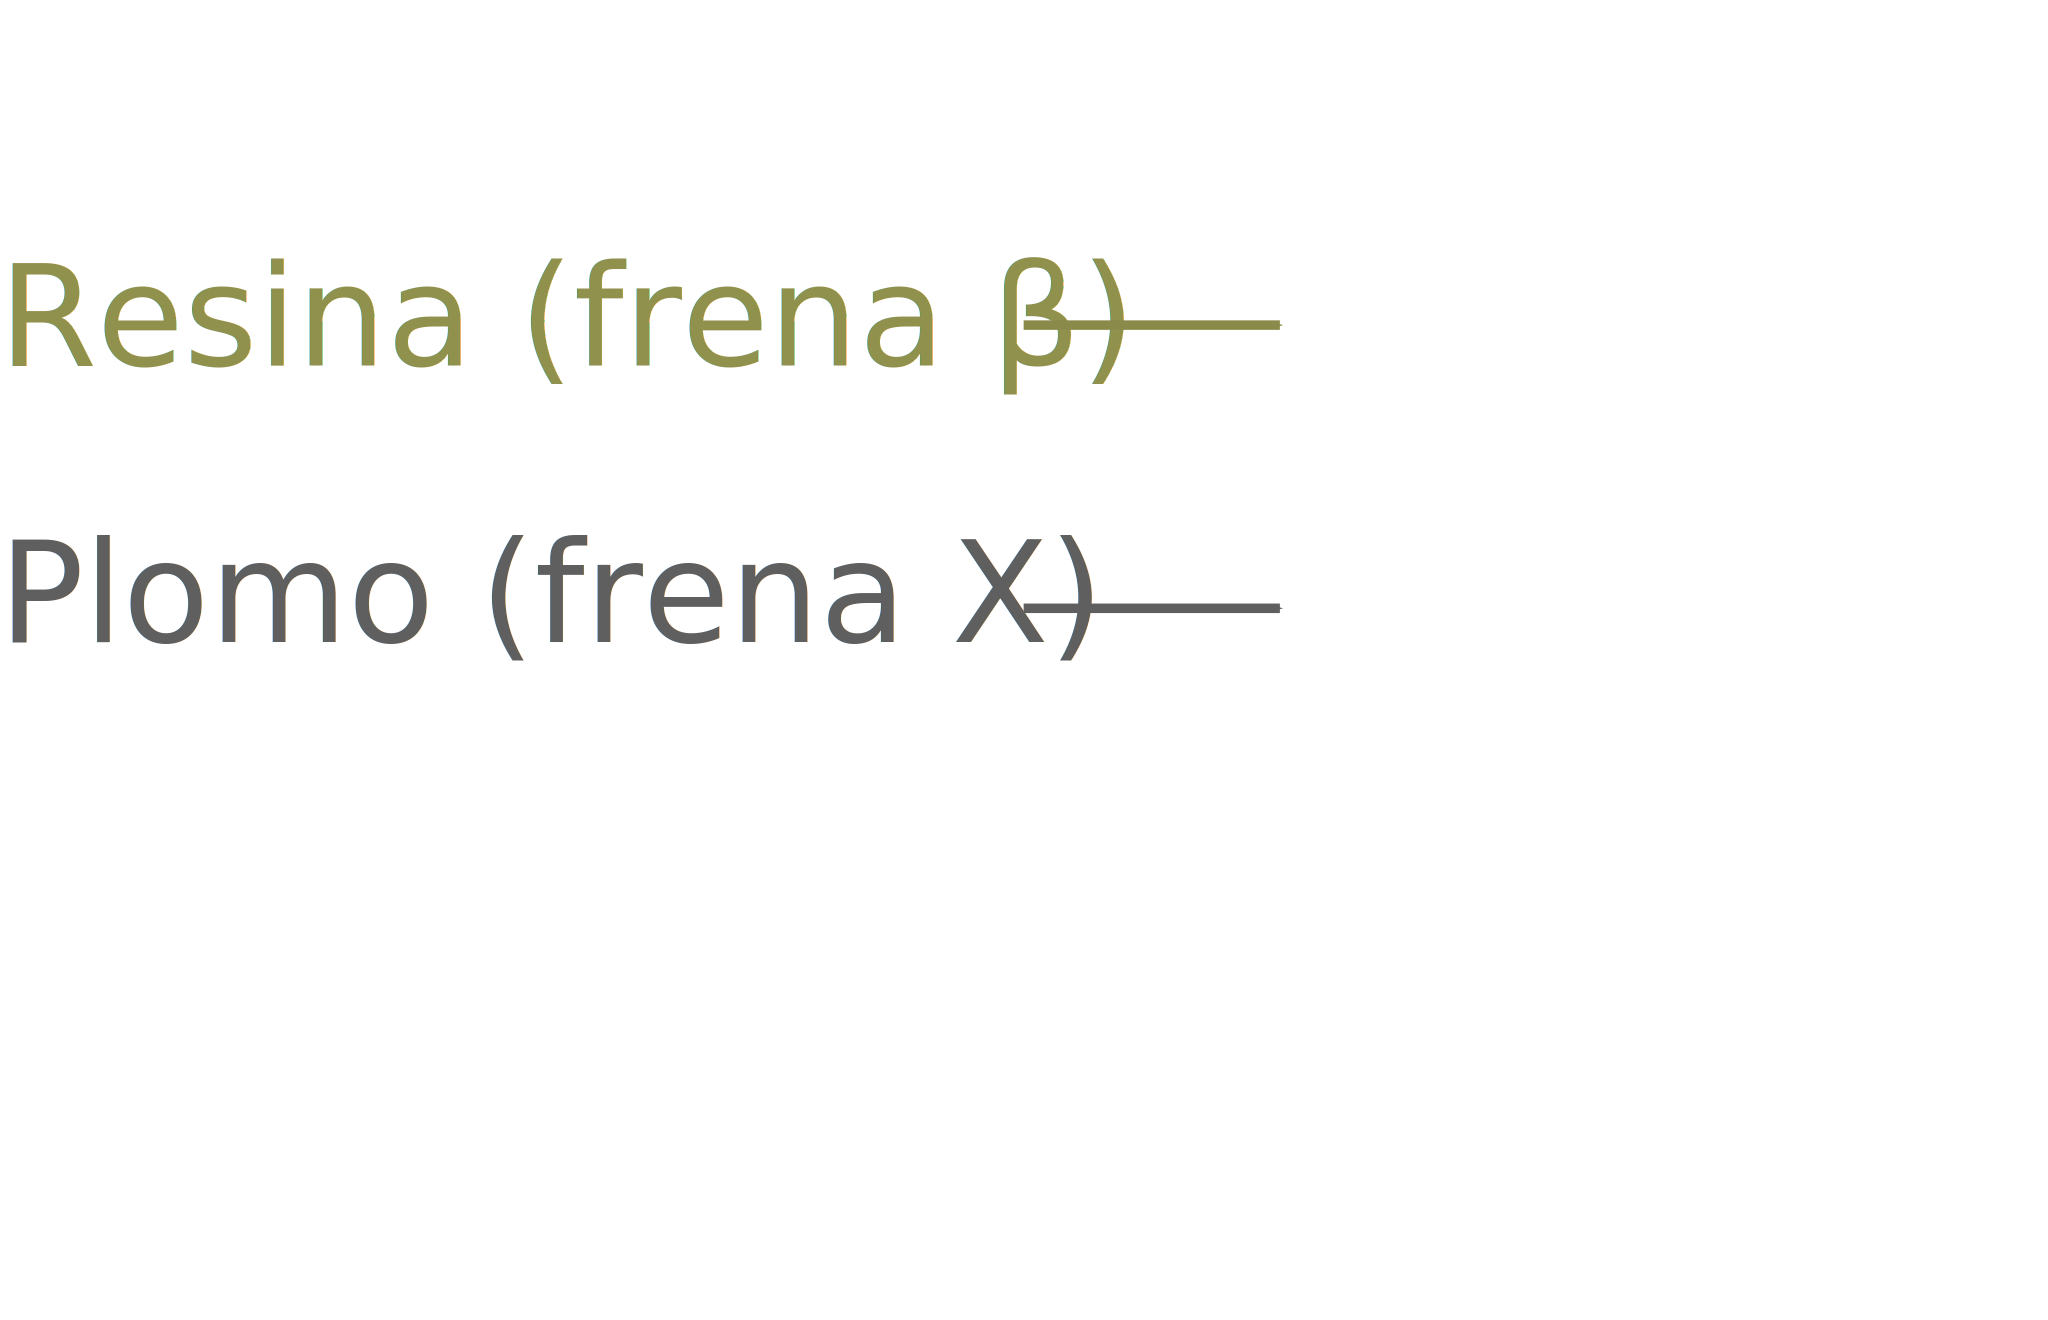
\includegraphics{figuras/poster/posicion_no.png}
        \caption{Safe position.}
        \label{fig:posicionno}
    \end{subfigure}
    \hspace{5mm}
    \begin{subfigure}[b]{.45\textwidth}
        \includegraphics{figuras/poster/posicion_si.png}
        \caption{Irradiation position.}
        \label{fig:posicionsi}
    \end{subfigure}
    \caption{Rotating assembly positions.}
    \label{fig:posicionespieza}
\end{figure}
\subsection{Construction}
\subsubsection{Walls}
Both ends of the cavity were covered with 
\SI{10}{\milli\meter} thick, \SI{90}{\milli\meter} diameter acrylic disks.

For the sidewalls, we were not able to find \SI{10}{\milli\meter} thick PVC pipe.
Initially we considered molding tubes out of paraffin or acrylic.
In the end, we decided to use two concentric PVC pipes,
filling the gap between them with acrylic.
\subsubsection{Rotating assembly}
The rotating assembly is made out of cast lead which was turned on a lathe
(\figref{fig:construccion_mariposa}).
\fig{construccion_mariposa}{figuras/irradiador/construccion_mariposa.pdf}
{Construction steps for the rotating assembly.
The turning step required a handle for the chuck to hold.
This handle was cut after turning.}
For the casting step, we turned to Abraham Murillo, from the
Escuela Técnica Nº 33 Fundicion Maestranza del Plumerillo.
The shop turned a wooden pattern slightly bigger than the desired final dimensions.
This was due to
\begin{itemize}
    \item the thermal contraction of lead when it cools down, and
    \item the extra thickness necessary for the final turning step.
\end{itemize}
We packed sand around the pattern in order to create a mold.
We added a vent hole for the hot gases to escape,
and a tube for the liquid metal to flow into the mold
(\figref{fig:moldeplomo}).
\fig{moldeplomo}{figuras/irradiador/molde_plomo.pdf}
{Cross section of the mold used for the rotating lead piece.
It was built out of sand packed around a wooden pattern.
The liquid metal was poured in through the tube on the right.
The hole on top provides a vent for hot gases.}
The resulting cast has a rough surface due to the sand grains in the mold.
In order to give it the exact dimensions we required,
and a smooth finish,
we received assistance from 
Eriel Fernandez from the FIUBA machine shop.
While we originally planned for a spherical piece,
this was not feasible on a manual lathe.
Instead, we settled for a piecewise linear cross-section
which covers the irradiator cavity
and is able to rotate within it
(\figref{fig:torneo_simple}).
\fig{torneo_simple}{figuras/irradiador/torneo_simple.pdf}
{We chose a shape simple enough to turn in a manual lathe,
which covers the irradiator cavity and is able to rotate within it.
The last requirement is met by ensuring the corners are within a circle
whose diameter matches the cavity's inner diameter.}
The final dimensions are in \figref{fig:torneo}.
The softness of the material required careful turning at low RPM.
\fig{torneo}{figuras/irradiador/torneo.pdf}
{Cross section of the rotating lead piece after turning (all dimensions are in mm).}
\subsubsection{Pocket for radiation source}
The radiation source is held in a plastic pocket.
Although the source has a threaded hole which can be used to secure it,
screwing it in would require close manipulation
and exposing someone's hands to radiation for a length of time.
Therefore, we decided to use a pocket such that the source
can be quickly dropped in without lengthy exposures to radiation.

We aimed to stop all electrons before they reach the lead piece.
Therefore, we shaped the plastic as a spherical cap which covers
the lead as much as possible,
while still being able to rotate inside the cavity.

Due to the difficulty in resin-casting a rounded shape with a cavity,
we turned to Iván G. Pollitzer from the
Laboratorio Abierto de Electrónica at FIUBA.
Iván guided us in designing a 3D printed ABS piece.
It consists of two parts printed separately
(\figref{fig:blender}),
\fig{blender}{figuras/irradiador/blender_small.png}
{The two parts that we 3D printed in ABS and glued together.
The space between the two parts forms a pocket where the radiation source is held.}
which we then filled with acrylic and glued together.

We screwed the plastic to the lead piece using headless screws,
drilling and tapping holes in both pieces.
\subsection{Radiation protection calculations}
%
\subsubsection{Bremsstrahlung calculations}
The $\beta$ particles emitted from the radiation source are stopped in plastic,
where they produce braking radiation.
We calculate its magnitude starting from the energy spectrum of the emitted electrons.
Because the source is in secular equilibrium (equal \Strontium and \Yttrium activities),
we sum their spectra taken from
Radiological Toolbox\cite{eckerman2006radiological}
and then normalize to the source's nominal activity, \SI{100}{\milli\curie}
(\figref{fig:actividadsr90}).
\fig{actividadsr90}{figuras/irradiador/actividad.pdf}
{Electron energy spectrum for a
\Strontium source whose activity is \SI{100}{\milli\curie}\cite{eckerman_icrp_2007}.}
We then calculate the bremstrahlung spectrum by integrating \equref{eq:kramers}
(\figref{fig:espectrox}).
\fig{espectrox}{figuras/irradiador/espectrox.pdf}
{Calculated bremsstrahlung spectrum in the PVC outer wall.}
%
\subsubsection{X ray shielding in lead}
We applied \equref{eq:absorcionx} 
using lead absorption coefficients published by NIST\cite{xraycoef},
resulting in the attenuated spectrum in \figref{fig:xatenuado}.
\fig{xatenuado}{figuras/irradiador/xatenuado.pdf}
{Calculated X ray spectrum in the irradiator's outer surface.}
% TODO: tasa de dosis final según distancia, comparar con mediciones
%
%
\subsubsection{Monte Carlo simulations with \Strontium source}
The \Strontium source emits electrons with a wide energy spectrum
(\figref{fig:actividadsr90}).
This is the sum of the emission spectra of \Strontium and \Yttrium.
We simulated this wide-spectrum electron beam directed perpendicularly into soft tissue,
logging the deposited energy as a function of depth
(\figref{fig:deposicionsr90}).
\fig{deposicionsr90}{figuras/montecarlo/deposicion_sr90.pdf}
{Energy deposited in soft tissue as a function of distance,
by an electron beam produced by a \Strontium source.}
In this way we fit an average mass stopping power 
$S/\rho$ (\figref{fig:stoppingsr90})
\fig{stoppingsr90}{figuras/montecarlo/stopping_sr90.pdf}
{Average mass stopping power of soft tissue for
electrons coming from a \Strontium source.
The cross marks the point at which the dose rate
matches the value tabulated in \cite{delacroix_radionuclide_2002}.}
which allows us to calculate surface dose rate using
\begin{align*}
    \dot D &= \frac{AS/\rho}{4\pi r^2}
\end{align*}
, with $A=\SI{100}{\milli\curie}$ the source's activity.
This calculated dose rate matches the value tabulated in 
\cite{delacroix_radionuclide_2002} if averaged down to a depth of
\SI{.35}{\milli\meter}.
This serves as a verification that our Monte Carlo simulations yield
results which are compatible with those in existing literature.
\subsubsection{Irradiator Monte Carlo simulations}
We are looking for an upper bound to the dose rate outside the irradiator.
If this value is within safe limits, it serves as a guarantee that
the irradiator is safe to operate.
As the thickness of lead is many times greater than the X ray attenuation length
($1/\mu$),
only a very small fraction of the incoming radiation can cross it.
Therefore, it is necessary to simulate a large number of electrons
emitted by the \Strontium source
in order to see an appreciable number exiting the irradiator.
This is itself necessary in order to have an accurate estimate of the dose rate.

One way to reduce the simulation CPU time is to use variance reduction
\cite{dressel_geometrical_2003}.
This is a technique used in Monte Carlo simulations 
which biases the random choices involved in propagating particles.
For example, it is possible to increase the probability that a particle will
travel through a wall without interacting, instead of scattering.
By keeping track of the likelihood of the particle's history,
it is possible to adjust its weight 
when calculating statistics like mean deposited energy.

This technique focuses simulation time in producing relevant events
(which lowers the estimator variances),
reducing the required processing power.

Given the difficulty in implementing variance reduction in Geant4,
we opted to speed up simulations by simplifying the geometry.
We simulated a spherically symmetric irradiator,
which consists of a \SI{10}{\milli\meter} acrylic shell 
surrounded by \SI{36}{\milli\meter} of lead (\figref{fig:corte_esferico}). 
\fig{corte_esferico}{figuras/irradiador/corte_esfera.png}
{Cutaway view of the simplified geometry used to simulate the irradiator in Geant4.}
All particles in the real irradiator have to cross at least those thicknesses of acrylic and lead.
Therefore, the dose in the real irradiator is guaranteed to be lower than in the simulated one.
Spherical symmetry allows us to ignore the dose angular distribution,
choosing instead to average over $\theta$ and $\phi$.
This drastically reduces the number of runs needed to reach an accurate estimate of the dose rate.
The results can be seen in \figref{fig:dosis_irradiador}.
\fig{dosis_irradiador}{figuras/montecarlo/dosis_irradiador.pdf}
{Monte Carlo results for energy deposition profile at the outer surface of the irradiator.}
The dose rate at the outer surface of the irradiator is
\SI{20.3}{\milli\sievert} per year.
This is a safe value when one takes into account that
people will mostly remain at a distance from the irradiator,
only touching it during brief periods of time.
